\documentclass[10pt]{article}
\usepackage{amsmath}
\usepackage{amssymb}
\usepackage{graphicx}
\usepackage{listings}
\usepackage{color}
\usepackage{float}
\usepackage{subcaption}
\usepackage{epstopdf}
\usepackage{url}
\usepackage{fullpage}
\usepackage{setspace}
\usepackage[usenames,dvipsnames,svgnames,table]{xcolor}
\usepackage{tikz}
\usetikzlibrary{shadows,arrows}
% Define the layers to draw the diagram
\pgfdeclarelayer{background}
\pgfdeclarelayer{foreground}
\pgfsetlayers{background,main,foreground}

% Define block styles
\tikzstyle{materia}=[draw, fill=blue!20, text width=6.0em, text centered,
  minimum height=1.5em]
\tikzstyle{practica} = [materia, text width=8em, minimum width=10em,
  minimum height=3em, rounded corners]
\tikzstyle{texto} = [above, text width=6em, text centered]
\tikzstyle{linepart} = [draw, thick, color=black!50, -latex', dashed]
\tikzstyle{line} = [draw, thick, color=black!50, -latex']
\tikzstyle{ur}=[draw, text centered, minimum height=0.01em]

% Define distances for bordering
\newcommand{\blockdist}{1.3}
\newcommand{\edgedist}{1.5}

\newcommand{\practica}[3]{node (p#1) [practica]
  {#2\\{\scriptsize\textit{#3}}}}

% Draw background
\newcommand{\background}[5]{%
  \begin{pgfonlayer}{background}
    % Left-top corner of the background rectangle
    \path (#1.west |- #2.north)+(-0.5,0.5) node (a1) {};
    % Right-bottom corner of the background rectanle
    \path (#3.east |- #4.south)+(+0.5,-0.25) node (a2) {};
    % Draw the background
    \path[fill=yellow!20,rounded corners, draw=black!50, dashed]
      (a1) rectangle (a2);
    \path (a1.east |- a1.south)+(0.8,-0.3) node (u1)[texto]
      {\scriptsize\textit{#5}};
  \end{pgfonlayer}}

\newcommand{\transreceptor}[3]{%
  \path [linepart] (#1.east) -- node [above]
    {\scriptsize #2} (#3);}


\usepackage[dvipsnames]{xcolor}

\usepackage{fancyvrb}

% redefine \VerbatimInput
\RecustomVerbatimCommand{\VerbatimInput}{VerbatimInput}%
{fontsize=\footnotesize,
 %
 frame=lines,  % top and bottom rule only
 framesep=2em, % separation between frame and text
 rulecolor=\color{Gray},
 %
 label=\fbox{\color{Black}output.txt},
 labelposition=topline,
 %
 commandchars=\|\(\), % escape character and argument delimiters for
                      % commands within the verbatim
 commentchar=*        % comment character
}

\begin{document}

\title{\textbf{Case Study [AE3T50]: \\Weight estimation tool for Commercial Transport Airplanes\\ "DOCUMENTATION"}}
\date{\today}
\author{Chy Lau\\ 4155955}
\maketitle
\thispagestyle{empty}
\clearpage

\tableofcontents
\thispagestyle{empty}
\clearpage
\setcounter{page}{1}
\section*{Terminology}

\textbf{Dictionary}\\
Python has something called a \textit{dictionary}, it is used in many other languages as well.
The dictionary is important for this program to store values from the XML file and several other things.
A dictionary is similar to an array, which has elements that can be accessed using index numbers.
For example the first element of the array a = ['apple', 'pear', 'orange'] can be accessed by a[0].
With a dictionary the index numbers are not limited to integers, but also can be strings.
An example of a dictionary is, b = \{'first': 'apple', 'second':'pear', 'three':'orange'\}, 'first' is called the \textit{key} and 'apple' is called the \textit{value}. To get the value 'apple', the corresponding key is specified, b['first'].
 \clearpage
\section{Introduction}
For document describes the code and how it is build up.
The code can be found in the delivered files and is also available online at \url{https://github.com/ChyLau/weviation/tree/master/weviation}.
Additionally, the logbook can be found at \url{https://github.com/ChyLau/weviation/commits/master} and gives a good indication of how much time is spend on this case study.

In Figure~\ref{fig:flow_bb} and~\ref{fig:flow_gui} the flow diagrams can be seen. Each diagram has three main parts: input, computation and output.
The input section is the same for both the black box and GUI, but they differ in the output part.
The black box can be used as a module for another project, and the GUI is for users.
For more customizability the GUI is used, which allows user interaction.

The following sections describe the parts of the flow diagram, starting with the Input (section~\ref{sec:input}), following with the Computation (section~\ref{sec:comp}) and ending with the Output (section~\ref{sec:output}).

Next the validation of the blackbox/GUI is described in section~\ref{sec:validation}, which check if each method gives a similar result.

\begin{figure}[h]
\centering
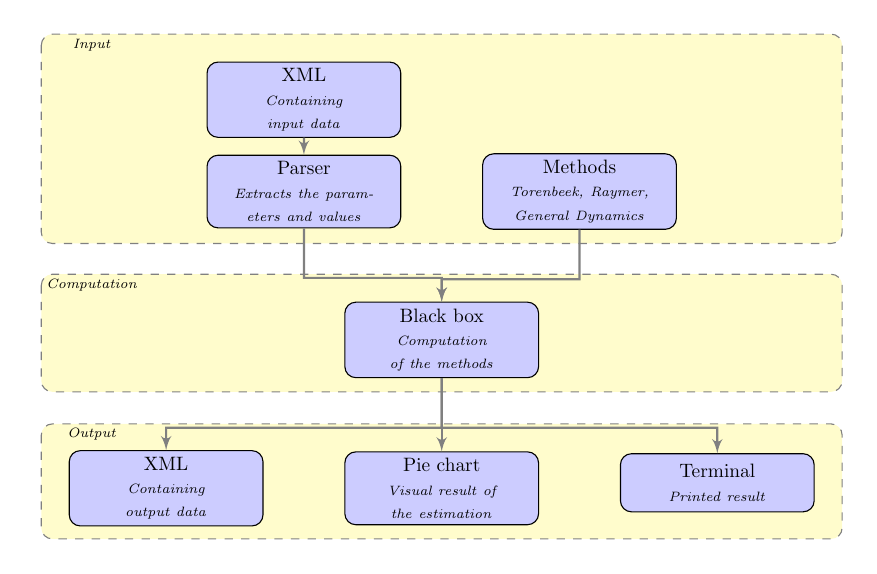
\begin{tikzpicture}[scale=0.7,transform shape]

  % Draw diagram elements
\path \practica{1}{Black box}{Computation of the methods};

\path (p1.north)+(-2.5,2.0) \practica{2}{Parser}{Extracts the parameters and values};
\path (p2.north)+(0.0,1.0) \practica{3}{XML}{Containing input data};

\path (p1.north)+(2.5,2) \practica{4}{Methods}{Torenbeek, Raymer, General Dynamics};

\path (p1.south)+(0.0,-2.0) \practica{5}{Pie chart}{Visual result of the estimation};
\path (p1.south)+(-5,-2.0) \practica{6}{XML}{Containing output data};
\path (p1.south)+(5,-1.9) \practica{7}{Terminal}{Printed result};

\path [line] (p1.south) -- node [above] {} (p5);
\path [line] (p1.south) -- +(0.0,-0.9) -- +(-5.0,-0.9) -- node [above, midway] {} (p6);
\path [line] (p1.south) -- +(0.0,-0.9) -- +(5.0,-0.9) -- node [above, midway] {} (p7);

\path [line] (p3.south) -- node [above] {} (p2);
\path [line] (p2.south) -- +(0.0, -0.9) -- +(2.5, -0.9) -- node [above, midway] {} (p1);
\path [line] (p4.south) -- +(0.0, -0.9) -- +(-2.5, -0.9) -- node [above, midway] {} (p1);
  % Draw arrows between elements
  %\path [line] (p1.south) -- node [above] {} (p2);

  %\path [line] (p2.south) -- +(0.0,-0.5) -- +(-2.5,-0.5)
  %  -- node [above, midway] {} (p3);
  %\path [line] (p3.south) -- node [above] {} (p5) ;

  %\path [line] (p2.south) -- +(0.0,-0.5) -- +(+2.5,-0.5)
  %  -- node [above, midway] {} (p4);
  %\path [linepart] (p3.east) -- +(+0.5,-0.0) -- +(+0.5,-1.75)
  %  -- node [left, midway] {} (p4);
  %\path [linepart] (p3.east) -- +(+0.5,-0.0) -- +(+0.5,-1.75)
  %  -- node [left, midway] {} (p4);

  %\path [line] (p4.south) -- +(0.0,-0.5) -- +(-2.5,-0.5)
  %  -- node [above, midway] {} (p6);
  %\path [line] (p5.south) -- +(0.0,-0.5) -- +(+2.5,-0.5)
  %  -- node [above, midway] {} (p6);
  %\path [linepart] (p2.east) -- +(2.75,0.0) -- +(2.75,-5.85)
  %  -- node [right] {} (p6);
  %\path [line] (p6.south) -- +(0.0,-0.25) -- +(-2.5,-0.25)
  %  -- node [above, midway] {} (p7);
  %\path [line] (p6.south) -- +(0.0,-0.25) -- +(+2.5,-0.25)
  %  -- node [above, midway] {} (p8);
  %\path [linepart] (p7.east) -- node [left] {} (p8);
  %\transreceptor{p8}{AM banda 40m}{ur1}

  %\path [line] (p7.south) -- node [above] {} (p9) ;
  %\path [line] (p8.south) -- node [above] {} (p10) ;
  %\path [linepart] (p9.east) -- node [left] {} (p10);
  %\transreceptor{p10}{CW}{ur2}
  %\path [line] (p9.south) -- node [above] {} (p11) ;
  %\path [line] (p10.south) -- node [above] {} (p12) ;
  %\path [linepart] (p11.east) -- node [left] {} (p12);
  %\transreceptor{p12}{FDMDV}{ur3}

  %\path [line] (p11.south) -- node [above] {} (p13) ;
  %\path [line] (p12.south) -- node [above] {} (p14) ;
  %\path [linepart] (p13.east) -- node [left] {} (p14);
  %\transreceptor{p14}{SSTV}{ur4}

  %\path [line] (p14.south) -- +(0.0,-0.5) -- +(-2.5,-0.5)
  %  -- node [above, midway] {} (p15);
  %\path [line] (p13.south) -- +(0.0,-0.5) -- +(+2.5,-0.5)
  %  -- node [above, midway] {} (p15);
  %\path [line] (p15.south) -- node [above] {} (p16) ;
  %\path [line] (p16.south) -- node [above] {} (p17) ;
  %\path [line] (p17.south) -- node [above] {} (p18) ;

  \background{p6}{p3}{p7}{p4}{Input}
  \background{p6}{p1}{p7}{p1}{Computation}
  \background{p6}{p5}{p7}{p5}{Output}
  %\background{p3}{p3}{p4}{p5}{II}
  %\background{p3}{p6}{p4}{p7}{III}
  %\background{p3}{p9}{p4}{p10}{IV}
  %\background{p3}{p11}{p4}{p12}{V}
  %\background{p3}{p13}{p4}{p14}{VI}
  %\background{p3}{p15}{p4}{p16}{VII}
  %\background{p3}{p17}{p4}{p17}{VIII}
  %\background{p3}{p18}{p4}{p18}{IX}
\end{tikzpicture}

\caption{Flow diagram for the black box.} \label{fig:flow_bb}
\end{figure}

\begin{figure}[h]
\centering
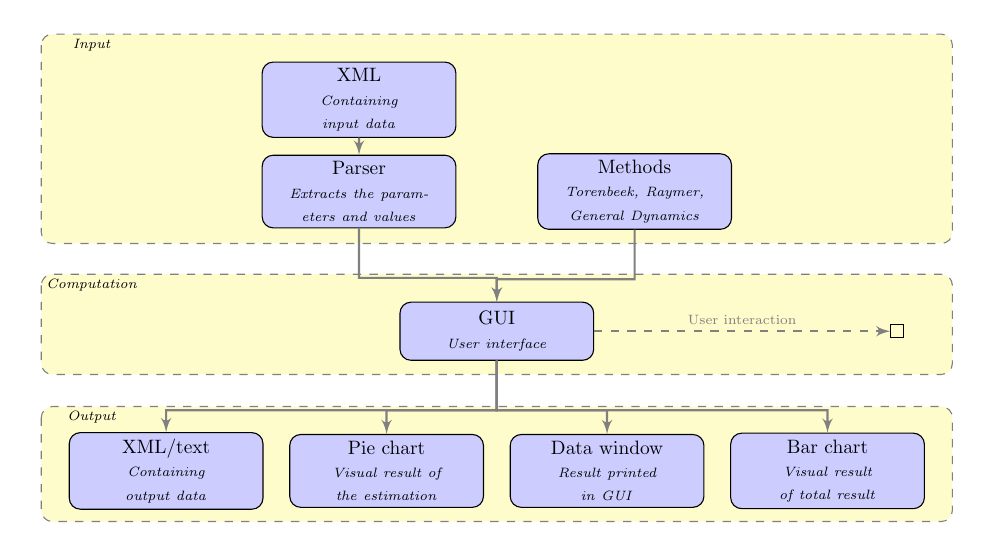
\begin{tikzpicture}[scale=0.7,transform shape]

  % Draw diagram elements
\path \practica{1}{GUI}{User interface};
\path (p1.east)+(+5.5,0) node (ur1)[ur] {};
\path (p1.north)+(-2.5,2.0) \practica{2}{Parser}{Extracts the parameters and values};
\path (p2.north)+(0.0,1.0) \practica{3}{XML}{Containing input data};

\path (p1.north)+(2.5,2) \practica{4}{Methods}{Torenbeek, Raymer, General Dynamics};

\path (p1.south)+(-2.0,-2.0) \practica{5}{Pie chart}{Visual result of the estimation};
\path (p1.south)+(-6,-2.0) \practica{6}{XML/text}{Containing output data};
\path (p1.south)+(2,-2.0) \practica{7}{Data window}{Result printed in GUI};
\path (p1.south)+(6,-2.0) \practica{8}{Bar chart}{Visual result of total result};

\path [line] (p1.south) -- +(0.0,-0.9) -- +(-2.0,-0.9) -- node [above, midway] {} (p5);
\path [line] (p1.south) -- +(0.0,-0.9) -- +(-6.0,-0.9) -- node [above, midway] {} (p6);
\path [line] (p1.south) -- +(0.0,-0.9) -- +(2.0,-0.9) -- node [above, midway] {} (p7);
\path [line] (p1.south) -- +(0.0,-0.9) -- +(6.0,-0.9) -- node [above, midway] {} (p8);

\path [line] (p3.south) -- node [above] {} (p2);
\path [line] (p2.south) -- +(0.0, -0.9) -- +(2.5, -0.9) -- node [above, midway] {} (p1);
\path [line] (p4.south) -- +(0.0, -0.9) -- +(-2.5, -0.9) -- node [above, midway] {} (p1);
\transreceptor{p1}{User interaction}{ur1}
  % Draw arrows between elements
  %\path [line] (p1.south) -- node [above] {} (p2);

  %\path [line] (p2.south) -- +(0.0,-0.5) -- +(-2.5,-0.5)
  %  -- node [above, midway] {} (p3);
  %\path [line] (p3.south) -- node [above] {} (p5) ;

  %\path [line] (p2.south) -- +(0.0,-0.5) -- +(+2.5,-0.5)
  %  -- node [above, midway] {} (p4);
  %\path [linepart] (p3.east) -- +(+0.5,-0.0) -- +(+0.5,-1.75)
  %  -- node [left, midway] {} (p4);
  %\path [linepart] (p3.east) -- +(+0.5,-0.0) -- +(+0.5,-1.75)
  %  -- node [left, midway] {} (p4);

  %\path [line] (p4.south) -- +(0.0,-0.5) -- +(-2.5,-0.5)
  %  -- node [above, midway] {} (p6);
  %\path [line] (p5.south) -- +(0.0,-0.5) -- +(+2.5,-0.5)
  %  -- node [above, midway] {} (p6);
  %\path [linepart] (p2.east) -- +(2.75,0.0) -- +(2.75,-5.85)
  %  -- node [right] {} (p6);
  %\path [line] (p6.south) -- +(0.0,-0.25) -- +(-2.5,-0.25)
  %  -- node [above, midway] {} (p7);
  %\path [line] (p6.south) -- +(0.0,-0.25) -- +(+2.5,-0.25)
  %  -- node [above, midway] {} (p8);
  %\path [linepart] (p7.east) -- node [left] {} (p8);
  %\transreceptor{p8}{AM banda 40m}{ur1}

  %\path [line] (p7.south) -- node [above] {} (p9) ;
  %\path [line] (p8.south) -- node [above] {} (p10) ;
  %\path [linepart] (p9.east) -- node [left] {} (p10);
  %\transreceptor{p10}{CW}{ur2}
  %\path [line] (p9.south) -- node [above] {} (p11) ;
  %\path [line] (p10.south) -- node [above] {} (p12) ;
  %\path [linepart] (p11.east) -- node [left] {} (p12);
  %\transreceptor{p12}{FDMDV}{ur3}

  %\path [line] (p11.south) -- node [above] {} (p13) ;
  %\path [line] (p12.south) -- node [above] {} (p14) ;
  %\path [linepart] (p13.east) -- node [left] {} (p14);
  %\transreceptor{p14}{SSTV}{ur4}

  %\path [line] (p14.south) -- +(0.0,-0.5) -- +(-2.5,-0.5)
  %  -- node [above, midway] {} (p15);
  %\path [line] (p13.south) -- +(0.0,-0.5) -- +(+2.5,-0.5)
  %  -- node [above, midway] {} (p15);
  %\path [line] (p15.south) -- node [above] {} (p16) ;
  %\path [line] (p16.south) -- node [above] {} (p17) ;
  %\path [line] (p17.south) -- node [above] {} (p18) ;

  \background{p6}{p3}{p8}{p4}{Input}
  \background{p6}{p1}{p8}{p1}{Computation}
  \background{p6}{p5}{p8}{p5}{Output}
  %\background{p3}{p3}{p4}{p5}{II}
  %\background{p3}{p6}{p4}{p7}{III}
  %\background{p3}{p9}{p4}{p10}{IV}
  %\background{p3}{p11}{p4}{p12}{V}
  %\background{p3}{p13}{p4}{p14}{VI}
  %\background{p3}{p15}{p4}{p16}{VII}
  %\background{p3}{p17}{p4}{p17}{VIII}
  %\background{p3}{p18}{p4}{p18}{IX}
\end{tikzpicture}

\caption{Flow diagram for the GUI.} \label{fig:flow_gui}
\end{figure}
 \clearpage
\lstset{
language=xml,
tabsize=3,
frame=lines,
label=code:xml,
%frame=framebox,
rulesepcolor=\color{gray},
xleftmargin=20pt,
framexleftmargin=15pt,
keywordstyle=\color{blue}\bf,
commentstyle=\color{OliveGreen},
stringstyle=\color{red},
numbers=left,
numberstyle=\tiny,
numbersep=5pt,
breaklines=true,
showstringspaces=false,
basicstyle=\footnotesize,
caption=XML file structure}

\section{Input}
\label{sec:input}
\subsection{XML}
\label{subsection:xml}
The input XML file \texttt{parameters.xml} contains the parameter and corresponding value for the functions.
Additionally, it specifies the information of the aircraft that those correspond to.
The basic syntax of an XML file is as follows, \texttt{\textless parameter \textgreater value \textless /parameter\textgreater}; for example \texttt{\textless n\_ult \textgreater 4.5 \textless/n\_ult\textgreater} specifies the ultimate load factor parameter with a value of 4.5.

Since the input data for three methods are in the XML file, there needs to be a structure.
The following structure is used for the XML file,
\lstinputlisting{code/structure.xml}
For multiple methods in one file, the method structure part is simply copied.

Some parameters are common in different methods, for example the ultimate load factor is present in all three methods.
These common parameters are specified for each method, so the ultimate load factor is specified three times.
The reason for this is to have more flexibility, if the user wants to test a different value for one method and keep the others the same this will be possible.

\subsection{Parser}
\label{sec:parser}
The XML parser \texttt{parse.py} extracts the parameters and values from the XML file and stores them into a dictionary.
Three dictionaries are used for the methods, input data from each method per dictionary.
The parser looks for the tags 'torenbeek', 'raymer' and 'gd' and stores the parameters and values under 'type' and 'component' into the dictionary.
Additionally, the information of the aircraft is stored in a separate dictionary.
To prevent duplicate elements in a method the parser checks everytime it adds a new element if the element already exists in the dictionary, if so, it will show an error.

\definecolor{Code}{rgb}{0,0,0}
\definecolor{Decorators}{rgb}{0.5,0.5,0.5}
\definecolor{Numbers}{rgb}{0.5,0,0}
\definecolor{MatchingBrackets}{rgb}{0.25,0.5,0.5}
\definecolor{Keywords}{rgb}{0,0,1}
\definecolor{self}{rgb}{0,0,0}
\definecolor{Strings}{rgb}{0,0.63,0}
\definecolor{Comments}{rgb}{0,0.63,1}
\definecolor{Backquotes}{rgb}{0,0,0}
\definecolor{Classname}{rgb}{0,0,0}
\definecolor{FunctionName}{rgb}{0,0,0}
\definecolor{Operators}{rgb}{0,0,0}
\definecolor{Background}{rgb}{1,1,1}

\lstnewenvironment{python}[1][]{
\lstset{
numbers=left,
numberstyle=\footnotesize,
numbersep=1em,
xleftmargin=1em,
framextopmargin=2em,
framexbottommargin=2em,
showspaces=false,
showtabs=false,
showstringspaces=false,
frame=l,
tabsize=4,
% Basic
basicstyle=\ttfamily\small\setstretch{1},
backgroundcolor=\color{Background},
language=Python,
% Comments
commentstyle=\color{Comments}\slshape,
% Strings
stringstyle=\color{Strings},
morecomment=[s][\color{Strings}]{"""}{"""},
morecomment=[s][\color{Strings}]{'''}{'''},
% keywords
morekeywords={import,from,class,def,for,while,if,is,in,elif,else,not,and,or,print,break,continue,return,True,False,None,access,as,,del,except,exec,finally,global,import,lambda,pass,print,raise,try,assert},
keywordstyle={\color{Keywords}\bfseries},
% additional keywords
morekeywords={[2]@invariant},
keywordstyle={[2]\color{Decorators}\slshape},
emph={self},
emphstyle={\color{self}\slshape},
%
caption=Torenbeek example function,
label=fig:methods
}}{}


\subsection{Methods}
\label{subsec:methods}
In \texttt{methods.py} functions for the three methods are specified, these functions are from literature (see references).
A class for each method provides a structure for the location of each function.
Functions can have arguments that set a coefficient to a specific value depending on the value of the argument.
For example in the Torenbeek functions there is the option to specify the unit system, imperial or SI.
Using an if-statement the unit system can be easily changed, see Listing~\ref{fig:methods}.
\clearpage
\begin{python}
def w_w(self, w_g, b_ref, Lambda, b, n_ult, s, t_r, unit):
    if unit == 'im':
            k_w = 0.0017
        elif unit == 'si':
            k_w = 0.00667
        else:
            print "USAGE: 'unit' is 'im' or 'si'."

        return k_w*w_g*(b_ref/cos(radians(Lambda)))**0.75*(1 + (b_ref*cos(radians(Lambda))/b)**0.5)*n_ult**0.55*(b*s/(w_g*t_r*cos(radians(Lambda))))**0.3
\end{python}


\section{Computation}
\label{sec:comp}

\subsection{Black box}
\label{subsec:blackbox}
The computation is done in the black box \texttt{blackbox.py}, which makes use of the input data and methods.
First the parser (see Section~\ref{subsec:parser}) is imported and then  called, which returns four dictionaries, with three of them containing data for the methods and one containing the aircraft information.
To use the functions described in the \texttt{methods.py} file it is first imported.
The arguments of the functions are set by specifying the key of the desired element, this is done for all of the functions.
The results of those functions are stored in dictionaries, one for each method, and are printed in the terminal/console window.
Additionally, the pie charts and output XML file are created using the dictionaries.
The pie charts are saved automatically as \texttt{pie\_tor.png}, \texttt{pie\_ray.png} and \texttt{pie\_gd.png} for Torenbeek, Raymer and General Dynamics, respectively.
The output XML file is saved as \texttt{output.xml.}




\subsection{GUI}
\label{subsec:gui}

The GUI \texttt{weviation.py} is made using wxPython, which is a library wrapper to create interfaces.
The interface allows users to have flexibility in calculating the weight by having more options.
The components to be calculated can be chosen, the unit for the input and output  parameters can be changed, the output can be exported as a text file and a bar chart is present.
The GUI is divided into three main sections: input window (left), output text window (middle), output visual window (right); see Figure~\ref{fig:gui1}.

The first step in creating a GUI is to come up with a simple layout.
A simple layout means having sections which are the same size, as less size configuration is needed, and therefore the three windows are the same in size.
The next step is the tabpanel in the left section, which is created using command called \texttt{wx.Notebook}.
Once a tab for each method is in place, the component selection and parameter value input are created with unit and type selection.
When the user hits the calculate button the program will first look at which methods are selected (in the bottom of the left section) and then look at which component(s) is selected and extract the non-empty values from the white text space, called text control (using wx.TextCtrl), and place them into a dictionary.
Similar to the black box (see Section~\ref{subsec:blackbox}) the functions from \texttt{methods.py} are imported.
All extracted values from the text control are converted to imperial units if unit selection is not imperial, since the functions expect values to be in imperial, and are put into the functions.
The results of those functions are put into a dictionary per method and are used for the output- and visual  window.

The output window section (middle) is essentially a large text control panel and it set to read-only to prevent alteration of the output values.
Before the values are printed in the text control, the name of the value and unit are added to it.
The text in the window is appended everytime the user hits calculate button and in order to clear the output window, the clear button can be pressed, which will set the value of the text control to "", which means empty.

In the visual output window (right) the dictionaries are used.
Similarily to the left section, tabs are used to display each pie chart and one bar chart.

\begin{figure}[ht]
\centering
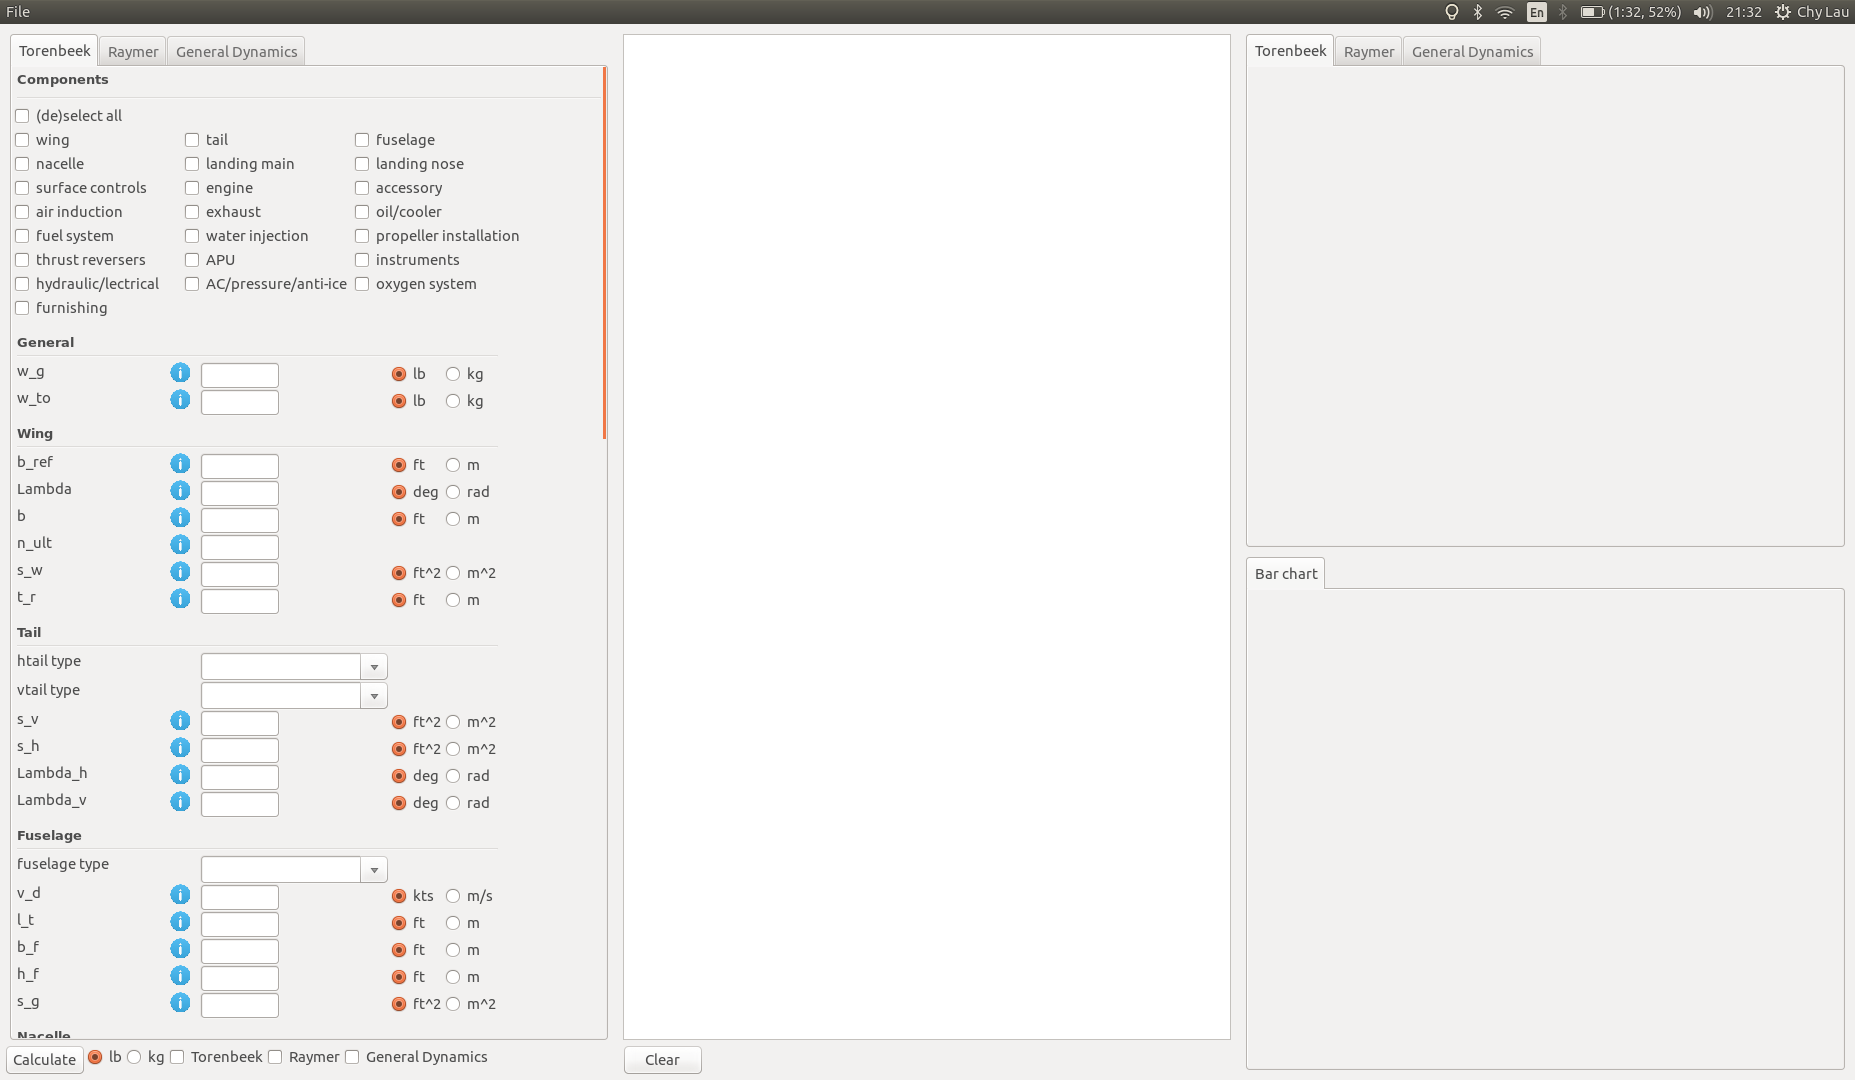
\includegraphics[width=1\textwidth]{image/gui_startup.png}
\caption{GUI on startup.}
\label{fig:gui1}
\end{figure}

In the file menu at the top, several options can be selected: load XML file, export to XML and export to text.
The load XML file option calls \texttt{parse.py} and sets the text control and combo box (type selection) to the parsed value.
Exporting to a XML/text file is done in the gui file and are saved as \texttt{output.xml} and \texttt{output.txt} for XML and text respectively.



\section{Output}
\label{sec:output}

\subsection{XML}


\subsection{Text (GUI)}
\label{subsec:text}
The output text file is generated in the GUI file.
Data in the output data window (middle) of the GUI is written to a .txt file.
This means that the text file contains exactly what is displayed in the output data window.
Again, the dialog function is called, which prompts a dialog message on completion.


\subsection{Bar- and pie chart (black box/GUI)}
\label{subsec:chart}
In the black box the pie charts are automatically saved for each function (see Section~\ref{subsec:blackbox}). Additionally, in the GUI a bar chart is generated, which presents the total weight of each method represented by different colours (Torenbeek: red, Raymer: green, GD: blue). For the GUI, however, the charts are not saved.

\subsection{Terminal and output data window (black box/GUI)}
\label{subsec:terminal}
For the black box the results are printed in the terminal/console window.
In the GUI the output data window shows results in a similar layout as in the terminal.

\section{Validation}
\label{sec:validation}
Most of the values are taken from the Civil Jet Aircraft Design website~\cite{data} and some other values are estimated or taken from other aircrafts.
The XML input file (provided) contains all the input values, the GUI can also be used to view the input values in a more user-friendly way.
The result of the weight estimation as the following (in Appendix~\ref{sec:outputxml} the output XML can be seen),
\VerbatimInput{code/output.txt}
What is noticable is that the total weight of Raymer is less than that of the other two.
The total weights of Torenbeek and General Dynamics are quite similar, 238,357 lb and 246,080 lb respectively.
The estimated weights under the structures group are quite similar for all three methods, however they simply differ in the propulsion and equipment group.
This is because parameter values in those groups are much harder to find or estimate and some are guessed.

Therefore, based on the results for the weight estimation, Torenbeek and General dynamics are more suitable.
\clearpage

\bibliographystyle{unsrt}
\bibliography{references}\clearpage
\appendix
\section{Output XML file}
\label{sec:outputxml}
\lstset{
    language=xml,
    tabsize=3,
    frame=lines,
    caption=Input XML file,
    label=code:sample,
    rulesepcolor=\color{gray},
    xleftmargin=20pt,
    framexleftmargin=15pt,
    keywordstyle=\color{blue}\bf,
    commentstyle=\color{OliveGreen},
    stringstyle=\color{red},
    numbers=left,
    numberstyle=\tiny,
    numbersep=5pt,
    breaklines=true,
    showstringspaces=false,
    basicstyle=\footnotesize,
    emph={general_dynamics, torenbeek, raymer, gd, unit, info, output},emphstyle={\color{magenta}}}

\lstinputlisting{code/output.xml}


\end{document}

